%%%%%%%%%%%%%%%%%%%%%%%%%%%%%%%%%%%%%%%%%
% Diaz Essay
% LaTeX Template
% Version 2.0 (13/1/19)
%
% This template originates from:
% http://www.LaTeXTemplates.com
%
% Authors:
% Vel (vel@LaTeXTemplates.com)
% Nicolas Diaz (nsdiaz@uc.cl)
%
% License:
% CC BY-NC-SA 3.0 (http://creativecommons.org/licenses/by-nc-sa/3.0/)
%
%%%%%%%%%%%%%%%%%%%%%%%%%%%%%%%%%%%%%%%%%

%%%%%%%%%%%%%%%%%%%%%%%%%%%%%%%%%%%%%%%%%
% Document Authors:
% Thijs van Boesschoten (t.van.boesschoten@protonmail.com)
%
%%%%%%%%%%%%%%%%%%%%%%%%%%%%%%%%%%%%%%%%%

%----------------------------------------------------------------------------------------
%	PACKAGES AND OTHER DOCUMENT CONFIGURATIONS
%----------------------------------------------------------------------------------------

\documentclass[11pt]{essayStyle} % Font size (can be 10pt, 11pt or 12pt)
\usepackage{listings}
%----------------------------------------------------------------------------------------
%	TITLE SECTION
%----------------------------------------------------------------------------------------

\title{\textbf{Industrial Automation} \\ {\Large\itshape Position and Temperature}} % Title and subtitle

\author{\textbf{Thijs van Boesschoten, Hussam Ayoub, Niousha Moshirzedeh} \\ \textit{Fontys University of Applied sciences}} % Author and institution

\date{\today} % Date, use \date{} for no date

%----------------------------------------------------------------------------------------

\begin{document}

\maketitle % Print the title section

%----------------------------------------------------------------------------------------
%	ABSTRACT AND KEYWORDS
%----------------------------------------------------------------------------------------

%\renewcommand{\abstractname}{Summary} % Uncomment to change the name of the abstract to something else

\begin{abstract}
This document will go through the process of automating an industrial process using industrial equipment in the form of PLCs.\\
This will entail the tools used for development, the design of the application and breakdown of the problem in states, using matlab to generate values for the PID system used in the program and binding it together using the Structured Text programming language.
\end{abstract}

\vspace{30pt} % Vertical whitespace between the abstract and first section

%----------------------------------------------------------------------------------------
%	Version Management
%----------------------------------------------------------------------------------------

\begin{table}[h] % [h] forces the table to be output where it is defined in the code (it suppresses floating)
	\centering
	\begin{tabular}{l l r}
		\multicolumn{2}{c}{Version Management} \\
		\cmidrule(r){1-3}
		Version & Changes & Reason \\
		\midrule
		v0.1 & All & First Draft \\
		\bottomrule
	\end{tabular}
\end{table}

%----------------------------------------------------------------------------------------
%	Table of Contents
%----------------------------------------------------------------------------------------

\tableofcontents

\pagebreak

%----------------------------------------------------------------------------------------
%	ESSAY BODY
%----------------------------------------------------------------------------------------

\section{Introduction}

For this project, a company assigned us to automate the process of a movable tank. The tank will be used to contain and mix liquids(chemicals) in a temperature controlled environment. 

The general tasks that the system should be able to fulfill are:
\begin{enumerate}
	\item Fill liquid A into the tank.
	\item Fill liquid B into the tank.
	\item Stir liquids A\&B while heated to a temperature setpoint.
	\item Move the tank to a position setpoint.
	\item Empty the tank.
	\item Return the tank to the default position.
\end{enumerate}


To fulfill these functionalities the following hardware is installed and can be manipulated by our program:
\begin{itemize}
	\item Value A, B \& C
	\item Stirrer
	\item Level Switch S1, S2 \& S3
	\item Heater
	\item Temperature Sensor
	\item Servo Motor
\end{itemize}

\begin{figure}[h]
	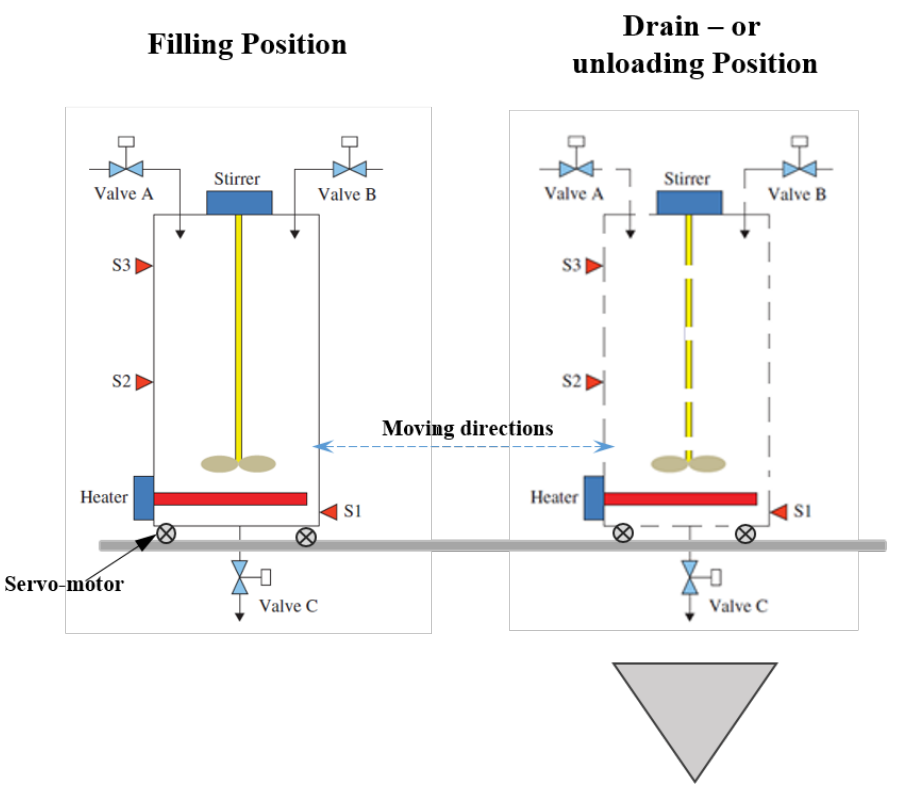
\includegraphics[width=\linewidth]{Tanks.png}
	\caption{Production set-up}
\end{figure}

%------------------------------------------------

\section{Tools \& Equipment}
For the development of our program, Twincat 3.0 will be used as the work that is provided will be in the form of a Twincat 3.0 archived project. Extracting this project shows that the basics like I/O and a base program has already been implemented. However this implementation is very crude and can use more refinement. In this manner, the first thing to be improved will be the visualization. 



\begin{figure}[h]
	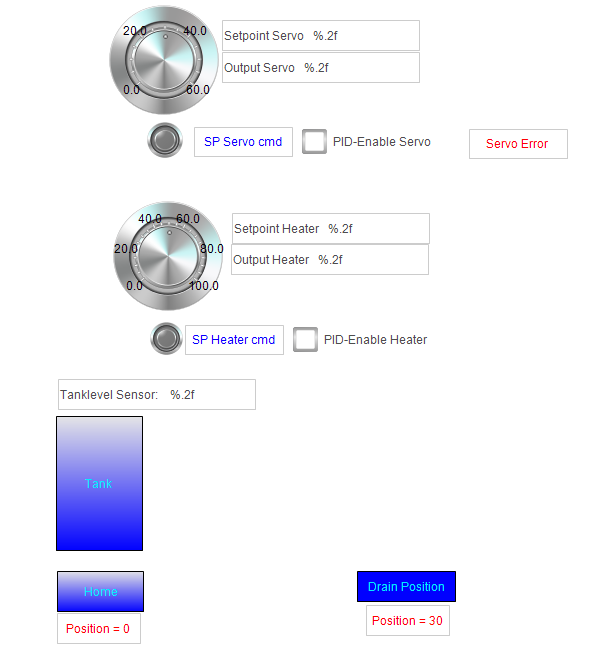
\includegraphics[width=\linewidth]{OldVisual.png}
	\caption{Old Visualization}
\end{figure}

Currently the UI is rather cluttered and not all information like the valves and stirrer are displayed. 

\begin{figure}[h]
	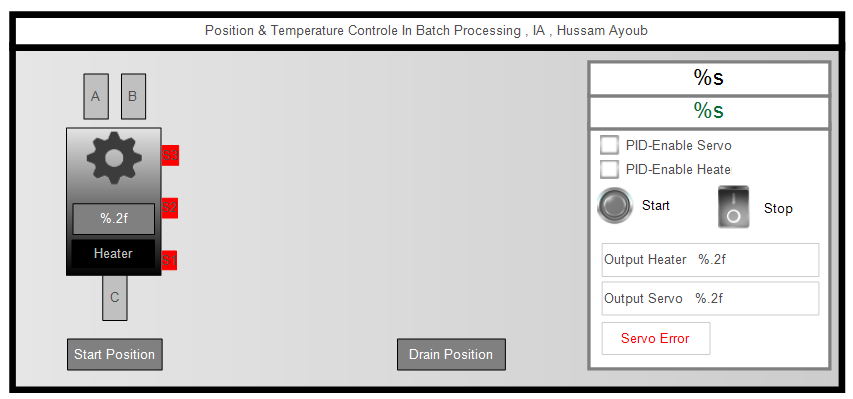
\includegraphics[width=\linewidth]{NewVisual.png}
	\caption{State Diagram of the process}
\end{figure}

As such a new visualization has been created to show all input information and the states of the outputs. 

%------------------------------------------------

\section{Program Design}

Having set the parameters of the project and a way to visualize the result, the process is the next thing in line. To start of has a state diagram been made to show the manner at which the program should operate given the criteria.

\begin{figure}[h]
	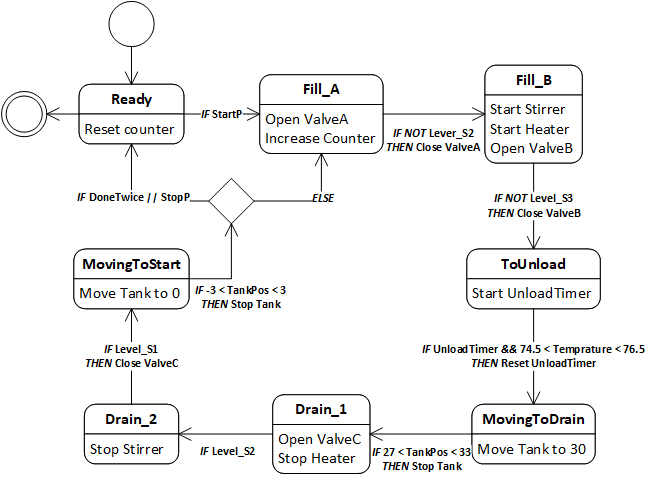
\includegraphics[width=\linewidth]{StateDiagram.png}
	\caption{New Visualization}
\end{figure}

Most of this code has already been implemented, the main section that needed to be filled in was the MAIN section which holds the state of the program, and the PID controller (fBDISCRETE$\_$PID) that needs to be completed.

%------------------------------------------------

\section{PID \& Matlab}
Starting with the PID controller needed for the movement of the tank to go fluently, the first part is to understand the system.

In the code is a transfer function given of $\frac{20}{0.5s^{2}+s}$. The transfer function can be used 
in Matlab with a PID controller to get the P, I and D values for out system. 
\begin{figure}[h]
	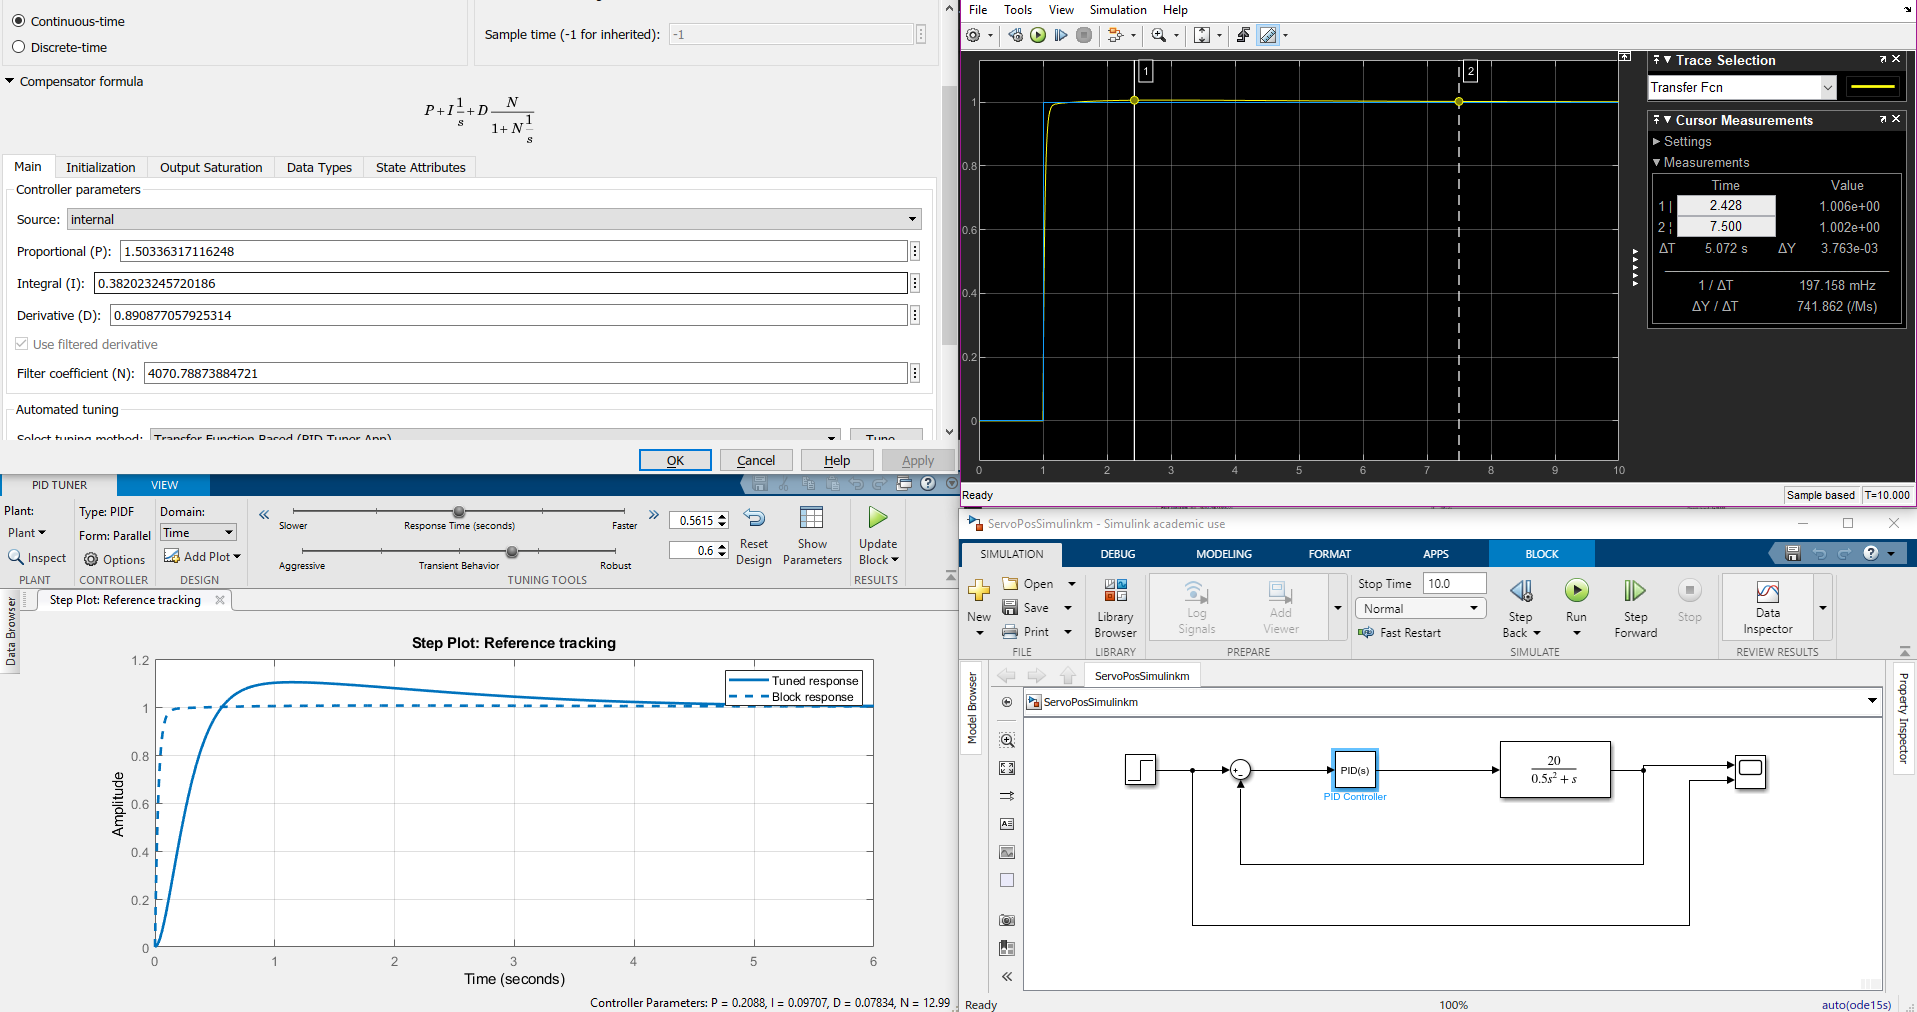
\includegraphics[width=\linewidth]{PIDTunedServo.png}
	\caption{PID Tuning for Servo}
\end{figure}

As can be seen in the image, the values of $P = 1.50336317116248$, $I = 0.382023245720186$ and $D = 0.890877057925314$ give an output that is fast and provides an overshoot that is within the 2\% overshoot allowed.

\begin{figure}[h]
	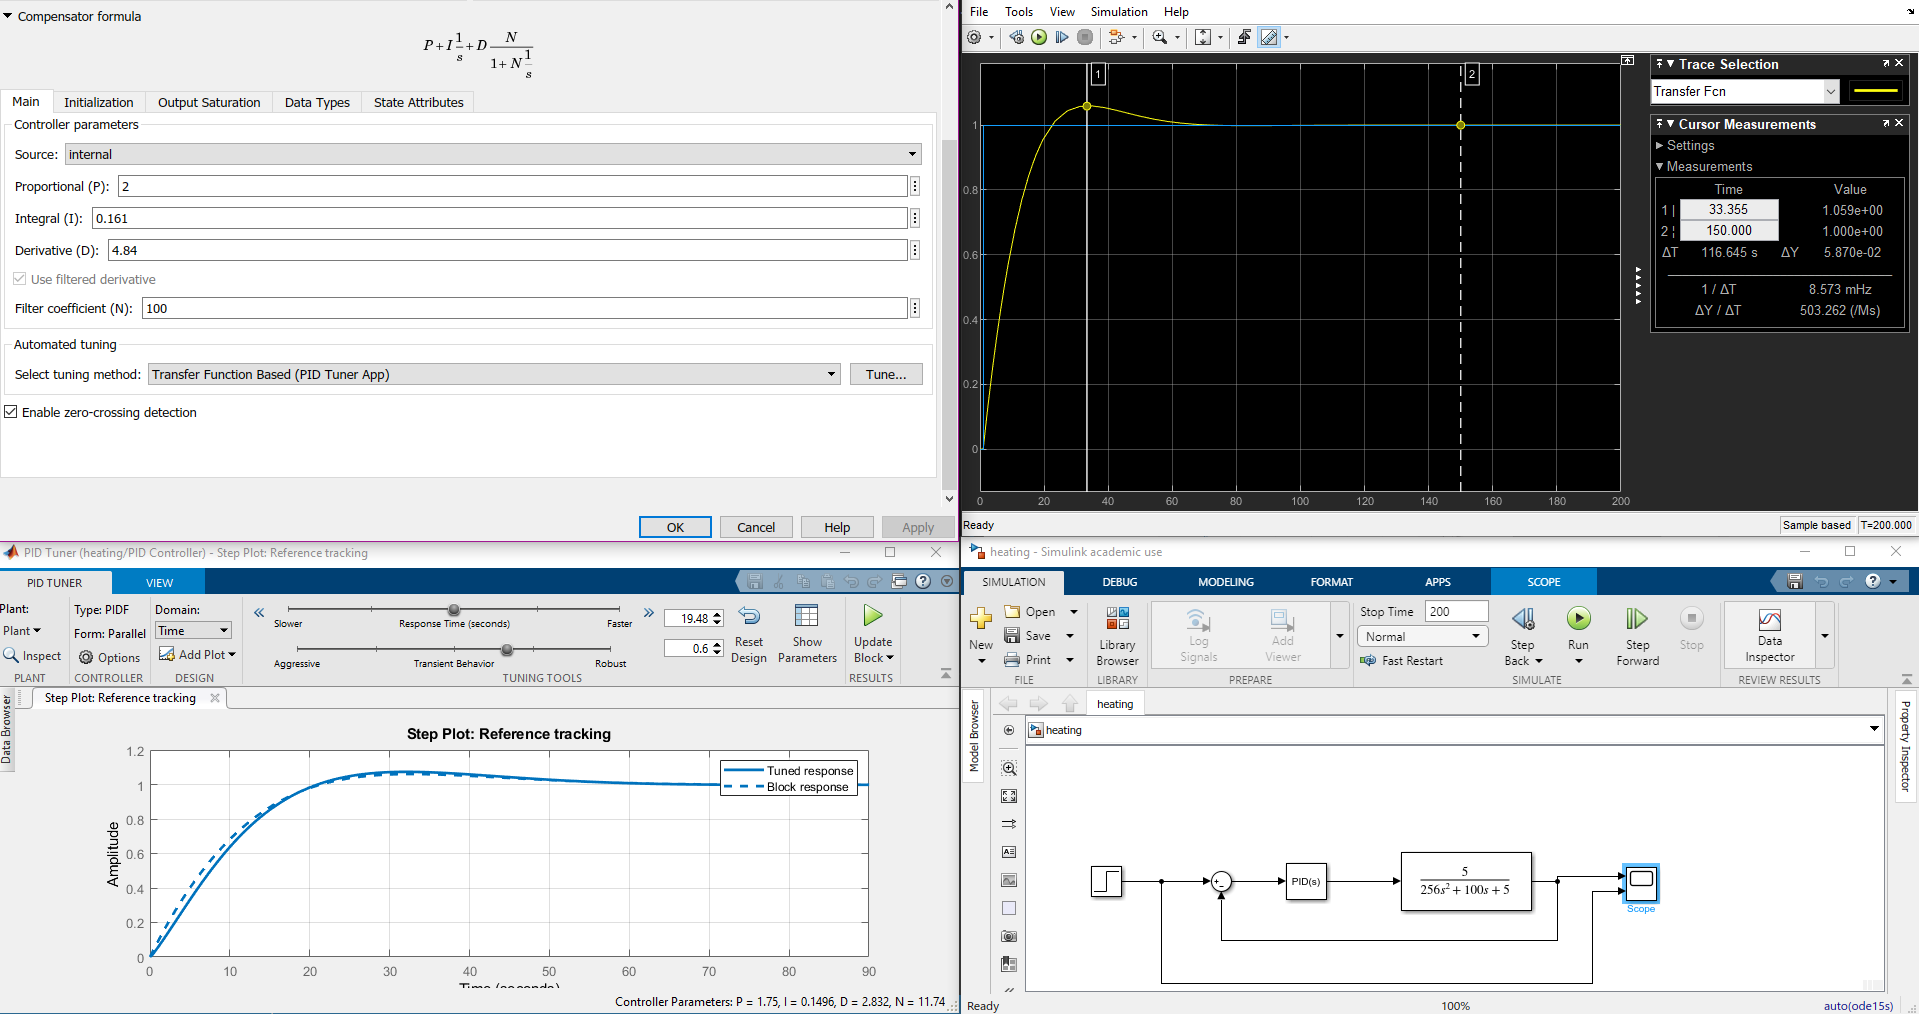
\includegraphics[width=\linewidth]{PIDTunedHeater.png}
	\caption{PID Tuning for Heater}
\end{figure}

Doing the same for the heater yields the values $P=2$, $I=0.161$ and finally $D=4.84$.

These values for the PID controllers come in useful, however can be utilized better by programmers in the "Advanced" PID - Algorithm \cite{Oswald:ia} form. $A=(k_{p}+k_{i}\frac{T}{2}+\frac{k_{d}}{T})$, $B=(-k_{p}+k_{i}\frac{T}{2}-\frac{2k_{d}}{T})$ and finally $C=\frac{k_{d}}{T}$

%------------------------------------------------

\section{Implementation}
With all the theoretical pieces together it is time to put things into action, starting of with the state machine in the MAIN file. Simply by using the following states programmed in:
\lstset{language=C++}
\begin{lstlisting}
TYPE SeqState :
(
	Ready,
	Fill_A,
	Fill_B,
	Heating,
	ToUnload,
	MovingToDrain,
	MovingToStart,
	Drain_1,
	Drain_2
);
END_TYPE
\end{lstlisting}

These programmed states can then be used in the main to go through in the form of a switch statement:

\begin{lstlisting}
CASE States OF // Sequence State
SeqState.Ready: 
	StateString := 'Ready!';
	Counter := 0; // sequence counter
	HeaterON := FALSE;
	IF GVL_IO.StartPr THEN // check if start button pressed
		States := SeqState.Fill_A; // go to state Fill A
	END_IF
	
SeqState.Fill_A: // sequence state fill A
	TotalStart := TRUE;
	...
\end{lstlisting}

Activating the Servo is done as follows:

\begin{lstlisting}
//
// *************  Servo with PID Controller  **************
//
IF (MoveTank AND NOT GVL_IO.xGenCtrl_Error ) THEN
	pidServo.Setpoint:=GVL_IO.SetPoint_ServoX;
END_IF

pidServo.Kp:= 1.503; // Kp parameter
 pidServo.Ki:= 0.382 ; // Ki parameter
 pidServo.Kd:= 0.89 ; // Kd parameter 

pidServo.MV_max_sat:= 10; // To protect Servo
pidServo.MV_min_sat:= -10; 
pidServo.xExt_Error:= Gvl_IO.xGenCtrl_Error;
pidServo.Yprocess:= LREAL_TO_REAL(GVL_IO.Output_ServoX);
pidServo(PID_enable:=PID_Servo_enable); 
\end{lstlisting}

This then leads into the fBDISCRETE\_PID function block which does the following to utilize the PID controller:

\begin{lstlisting}
Perr:= Setpoint - Yprocess;

A := (Kp + Ki * (Tsample/2) + (Kd/Tsample));
B := (-Kp + Ki *(Tsample/2) - (2*Kd/Tsample));
C :=  Kd/Tsample;

Mv_out:= prevMV_out +  A*Perr + B * Perr1 + C * Perr2;

// Update  samples 
prevMV_out := MV_out; // prevMV_out = MV_out[k-1] 
Perr2 := Perr1;       // e[k-2]
Perr1 := Perr;        // e[k-1]

\end{lstlisting}

%----------------------------------------------------------------------------------------
%	BIBLIOGRAPHY
%----------------------------------------------------------------------------------------

\bibliographystyle{unsrt}

\bibliography{refrences.bib}

%----------------------------------------------------------------------------------------

\end{document}
